\chapter{Risk Assessment}
\label{chap:riskAssesment}


%maybe some other potential thread should replace DDoS as it seems super unlikely for our business.
\section{DDoS}
\textbf{Description:} MjøsTaxi is widely known across Oppland, and therefore is a possible target for script kiddies, but also to competitors who want to disrupt our services.  \\
\textbf{Likelihood:} Unlikely. \\
\textbf{Impact:} A DDoS attack large enough to take down both the links to the HQ is likely not to last for too long. However, if the attacker plans ahead, an attack during a high-traffic time could have an impact. \\
\textbf{Mitigation:} Paying for DDoS protection from the ISP is a possibility, as this is an expensive solution to a likely insignificant problem, this is seen as unnecessary.

\section{Losing Connection to HQ}
\textbf{Description:} Problem that might occur while the network is available again is a flood of data which might result in a denial of service. \\
\textbf{Likelihood:} Unlikely\\
\textbf{Impact:} Drivers lose ability to get orders from headquarters and are only able to pick up fares "old-fashioned way", through cellphone calls and by being contacted in person. Also branches lose their access to internal applications, resulting in slowdown in workflow. \\
\textbf{Mitigation:} Having redundant connections from the HQ to the ISP, as well as having the old system in place as a backup.

\section{Losing Power at HQ}
\textbf{Description:} Losing power at our Headquarters due to events that are out of companies hands is always a possibility.  \\
\textbf{Likelihood:} Likely \\
\textbf{Impact:} Losing power at headquarters would mean that MjøsTaxi infrastructure is going down instantly. Shutting down in such a drastic manner introduces problems such as loss of data and possibility of damaged equipment.\\
\textbf{Mitigation:} Using UPS for critical parts of MjøsTaxi infrastructure to have enough power as back up and make sure neither data nor equipment is damaged. \cite{poweroutage}

\section{Phishing Attacks}
\textbf{Description:} While being a relatively big company in Norway, MjøsaTaxi is an obvious target for phishing attacks.  \\
\textbf{Likelihood:} Very likely\\
\textbf{Impact:} Depending on the scale of the phishing attack the impact can vary in loss of funds, data and potentially bad reputation.\\
\textbf{Mitigation:} Training for employees in regards of email and phone safety.

% Imma fix this later, because fuck Excel export lmao.
\section{Risk Assessment Matrix}
\begin{figure}[h]
\centering
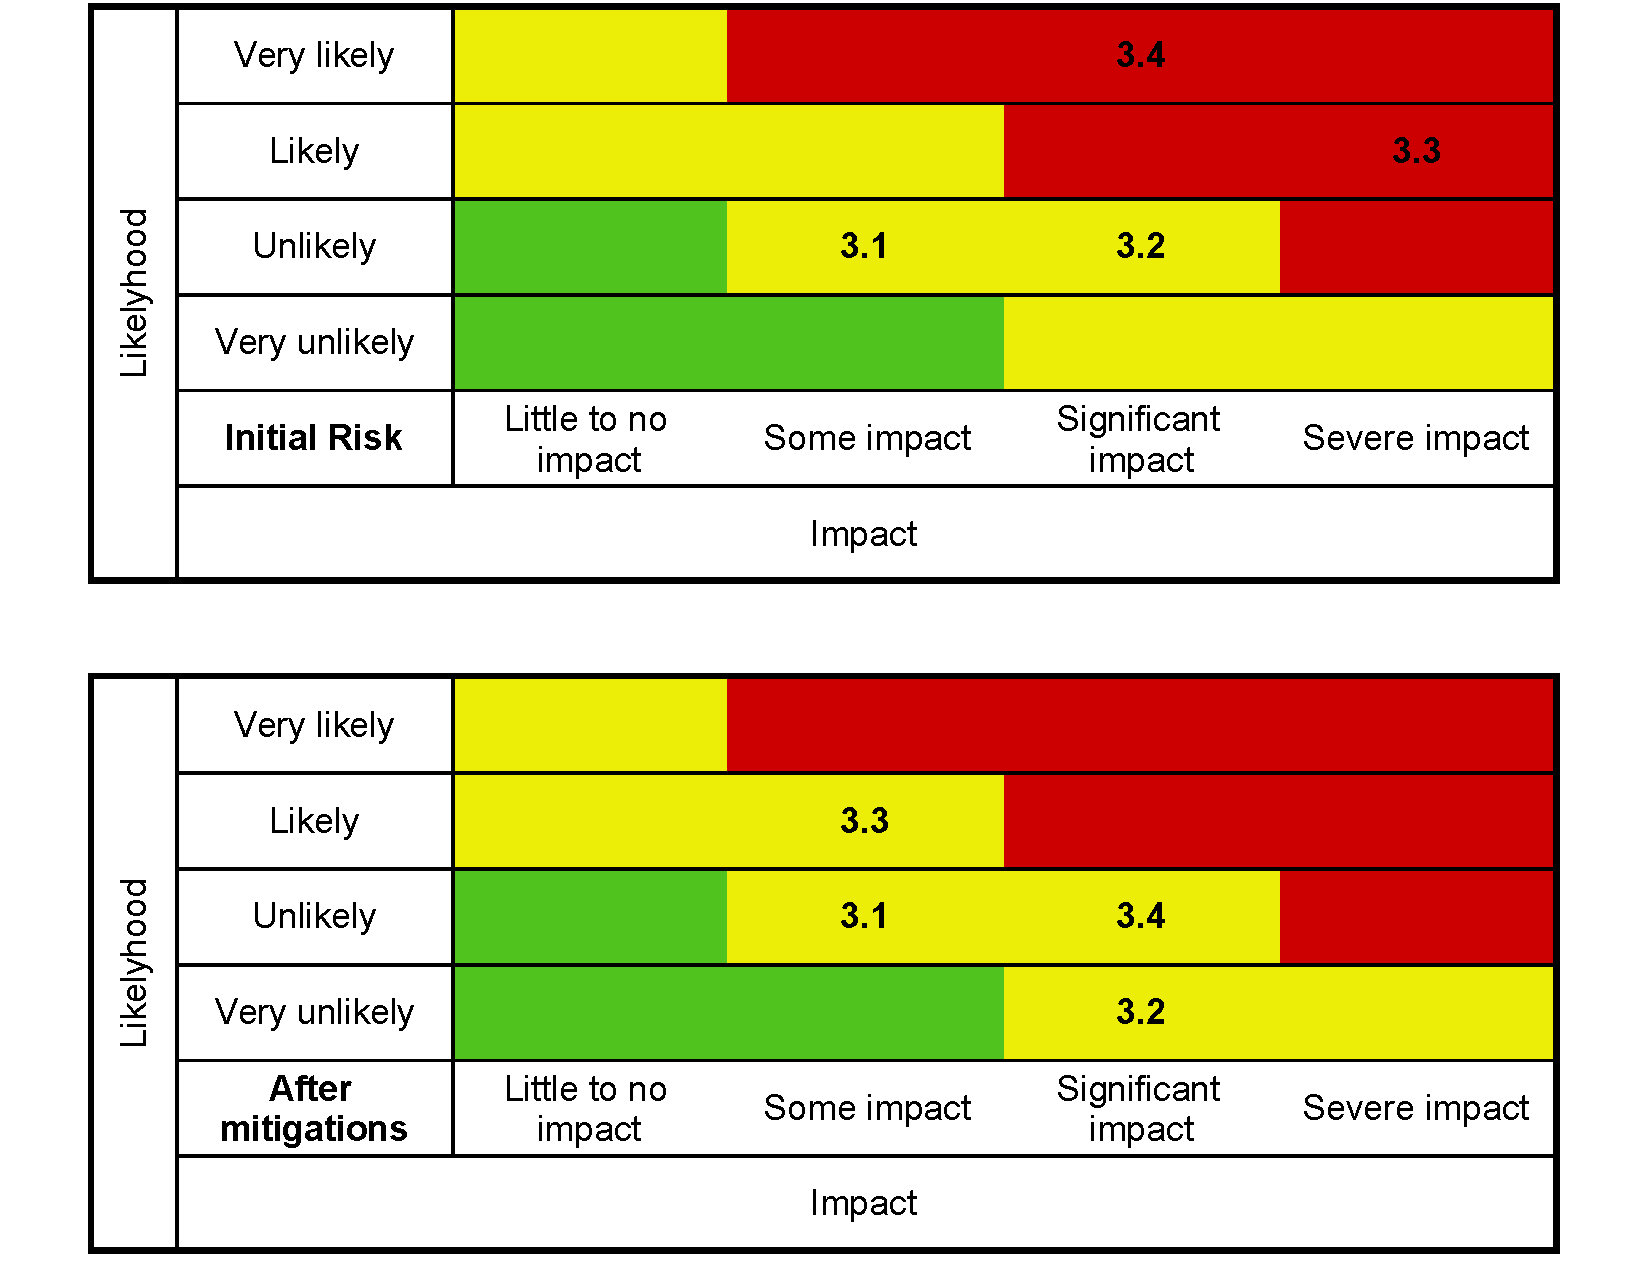
\includegraphics[width=0.9\textwidth]{fig/riskMatrix.pdf}
\caption{\label{fig:RiskMatrix}Risk assessment matrix before and after mitigation.}
\end{figure}

%\section{Ransomware}
%\textbf{Description:} \\
%\textbf{Likelihood:} \\
%\textbf{Impact:} \\
%\textbf{Mitigation:}